The proposed rover and \ac{SA} configurations for both mission sites are modeled with Blender/Phobos and loaded into MARS for mission scenario simulation. Phobos is ``an add-on for the open-source 3D modeling software Blender that enables the creation of robot models for use in robot frameworks like ROS and ROCK or in real-time simulations such as MARS'' \citeother{Phobos}. MARS is ``a cross-platform simulation and visualisation tool created for robotics research. It consists of a core framework containing all main simulation components, a GUI (based on Qt), 3D visualization (using OSG) and a physics engine (based on ODE)'' \citeother{MARSSim}. \refFig{fig:simulated-mission-site-ismenius-cavus} shows the robot model loaded on the MARS platform to simulate mission scenarios using a \ac{HiRISE} \ac{DTM} of a well preserved crater at Ismenius Cavus. The simulated solar power output data is produced by a \ac{PMS} implemented as part of this thesis and is integrated with the robot simulation toolkit.

\vspace{0.2cm}

\begin{figure}[h]
  \captionsetup[subfigure]{justification=centering}
  \centering
  \hypersetup{linkcolor=captionTextColor}
  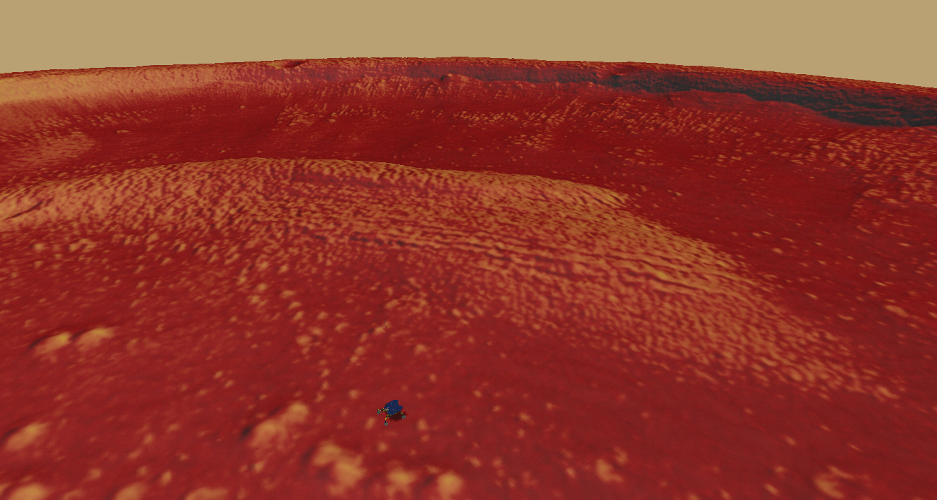
\includegraphics[width=0.9\linewidth]{sections/power-system-design/simulation/images/mars-sim-ismenius-cavus.png}\\
  \caption[Simulation of the rover inside a well preserved crater at Ismenius Cavus]
          {Simulation of the rover inside a well preserved crater at Ismenius Cavus.}
  \label{fig:simulated-mission-site-ismenius-cavus}
\end{figure}

\subsection{Z-Axis Revolutions}

\refFig{fig:sub:simulation-data-rover-revolution-generated-power-line-chart} and \refFig{fig:sub:simulation-data-rover-revolution-generated-power-polar-chart} are two different representations of the same solar power output obtained from commanding the rover to execute a \SI{10}{\degree} forward body-pitch followed by several revolutions around its z-axis. These revolutions result in a sinusoidal power output variation. Local spikes and dips are noted during the 480-\SI{600}{\second} and 840-\SI{960}{\second} time frames when the solar arrays are directed northwards. These are caused by the rover driving over uneven terrain which affect the \ac{SA} inclination and orientation. In \refFig{fig:sub:simulation-data-rover-revolution-generated-power-polar-chart}, the angle values represent the direction faced by the inclined \ac{SA}. Maximum power is generated when the \ac{SA} is oriented soutwards, towards the equator, in the general direction of the Sun. Inversely, facing northwards, away from the sun, generates the least amount of power.

\clearpage
\begin{figure}[h]
\captionsetup[subfigure]{justification=centering}
%\vspace{-2ex}
	\centering
    %% setup sizes
    \setlength{\subfigureWidth}{0.50\textwidth}
    \setlength{\graphicsHeight}{70mm}
    %% kill hyper-link highlighting
    \hypersetup{hidelinks=true}%
    %% the figures
    \begin{subfigure}[t]{\subfigureWidth}
        \centering
        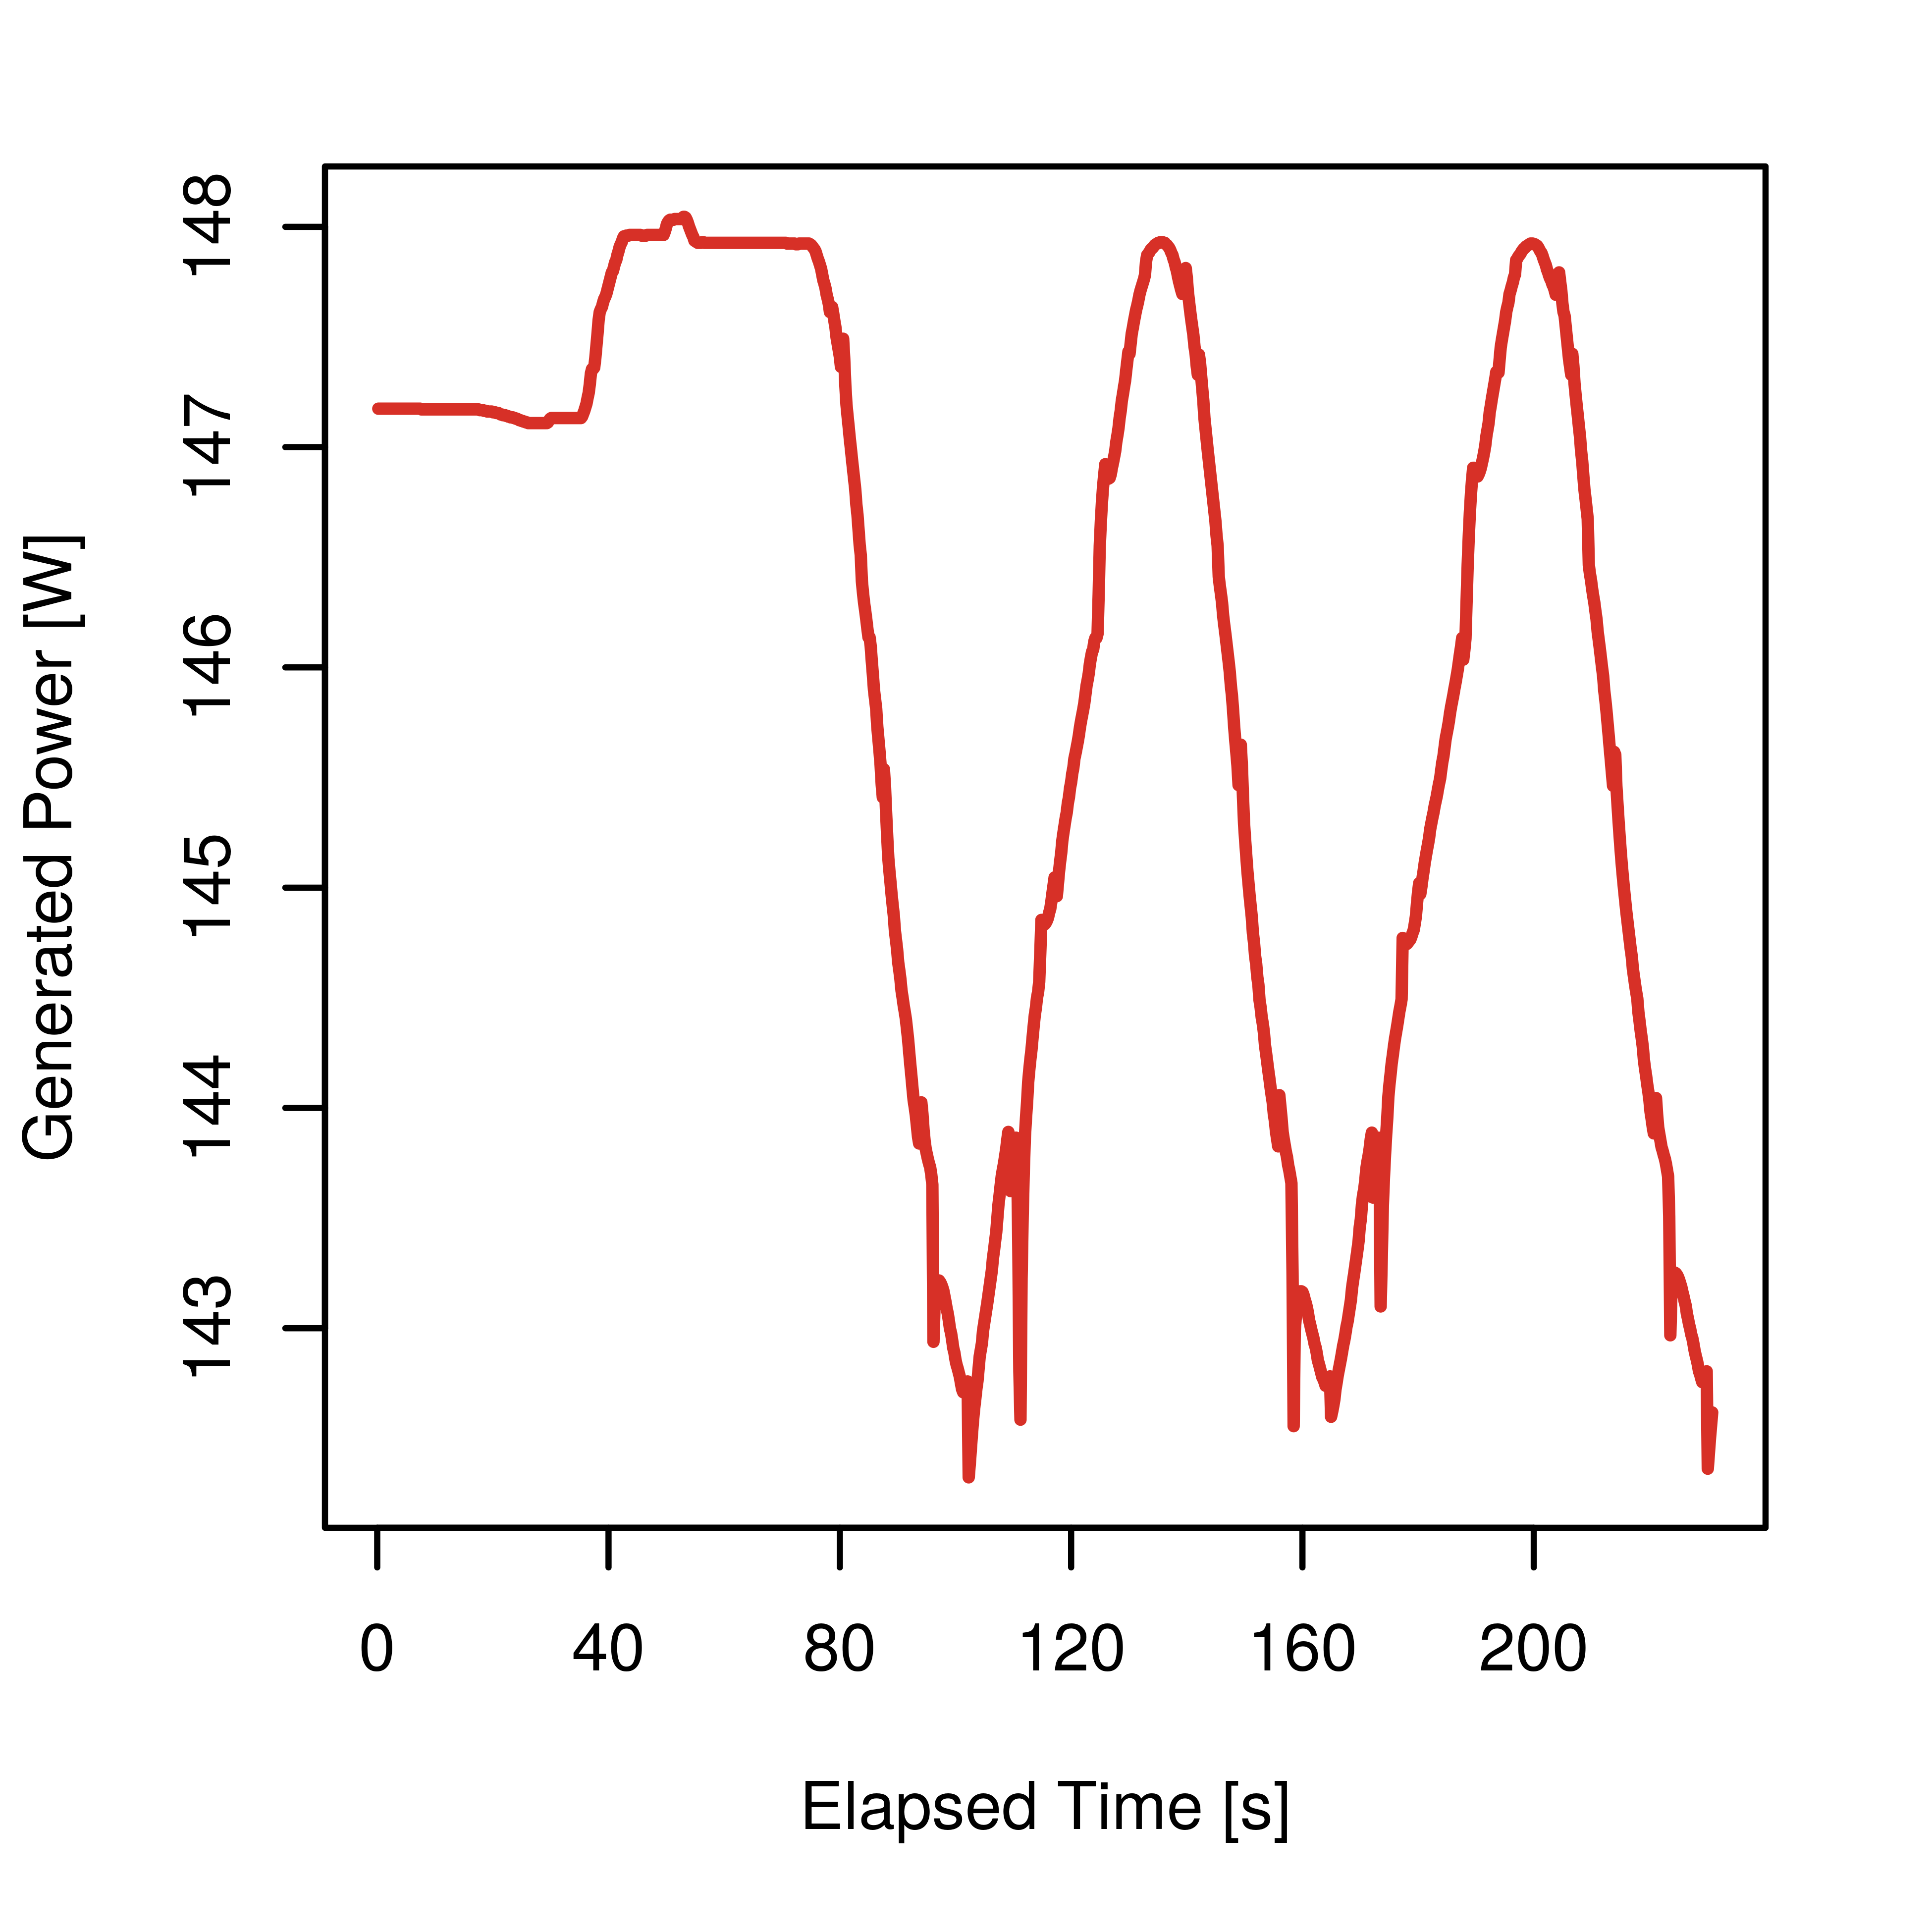
\includegraphics[height=\graphicsHeight]{sections/power-system-design/simulation/plots/zaxis-revolutions.png}
  		\subcaption{Line chart}
		\label{fig:sub:simulation-data-rover-revolution-generated-power-line-chart}
    \end{subfigure}\hfill
    \begin{subfigure}[t]{\subfigureWidth}
        \centering
        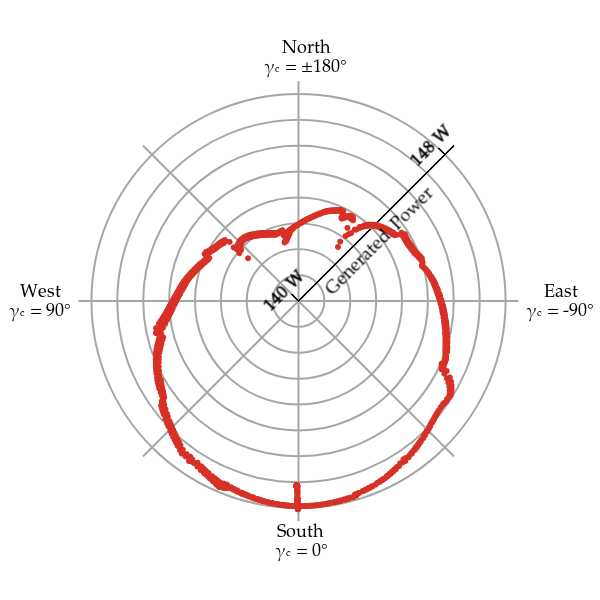
\includegraphics[height=\graphicsHeight]{sections/power-system-design/simulation/plots/zaxis-revolutions-polar.png}
  		\subcaption{Polar chart}
		\label{fig:sub:simulation-data-rover-revolution-generated-power-polar-chart}
	\end{subfigure}\\[0.6ex]
    \caption[Power generated by the rover's solar array for multiple revolutions along its z-axis]
            {Power generated by the rover's solar array for multiple revolutions along its z-axis. Simulation conditions is solar noon at Ismenius Cavus with $\beta \approx \SI{10}{\degree}$. In the polar chart, angle values represent the direction faced by the inclined solar array where \SI{0}{\degree} is South (towards the equator), \SI{-90}{\degree} is East, \SI{180}{\degree} is North, and \SI{90}{\degree} is West.}
    \label{fig:simulation-data-rover-revolution-generated-power}
\vspace{-2ex}
\end{figure}


\subsection{Slope Compensation}

The slope compensation scenario illustrated in \refFig{fig:sub:rover-on-slope-beta-small} is simulated in \refFig{fig:sub:rover-slope-compensation-simulation} where the rover's body is pitched bakwards by \SI{10}{\degree} while on a \SI{30}{\degree} forward inclined slope. The slope's inclination is facing away from the Sun, resulting in a worst case power output.

\begin{figure}[h]
\captionsetup[subfigure]{justification=centering}
\vspace{-4ex}
	\centering
    %% setup sizes
    \setlength{\subfigureWidth}{0.50\textwidth}
    \setlength{\graphicsHeight}{74mm}
    %% kill hyper-link highlighting
    \hypersetup{hidelinks=true}%
    %% the figures
    \begin{subfigure}[t]{\subfigureWidth}
        \centering
        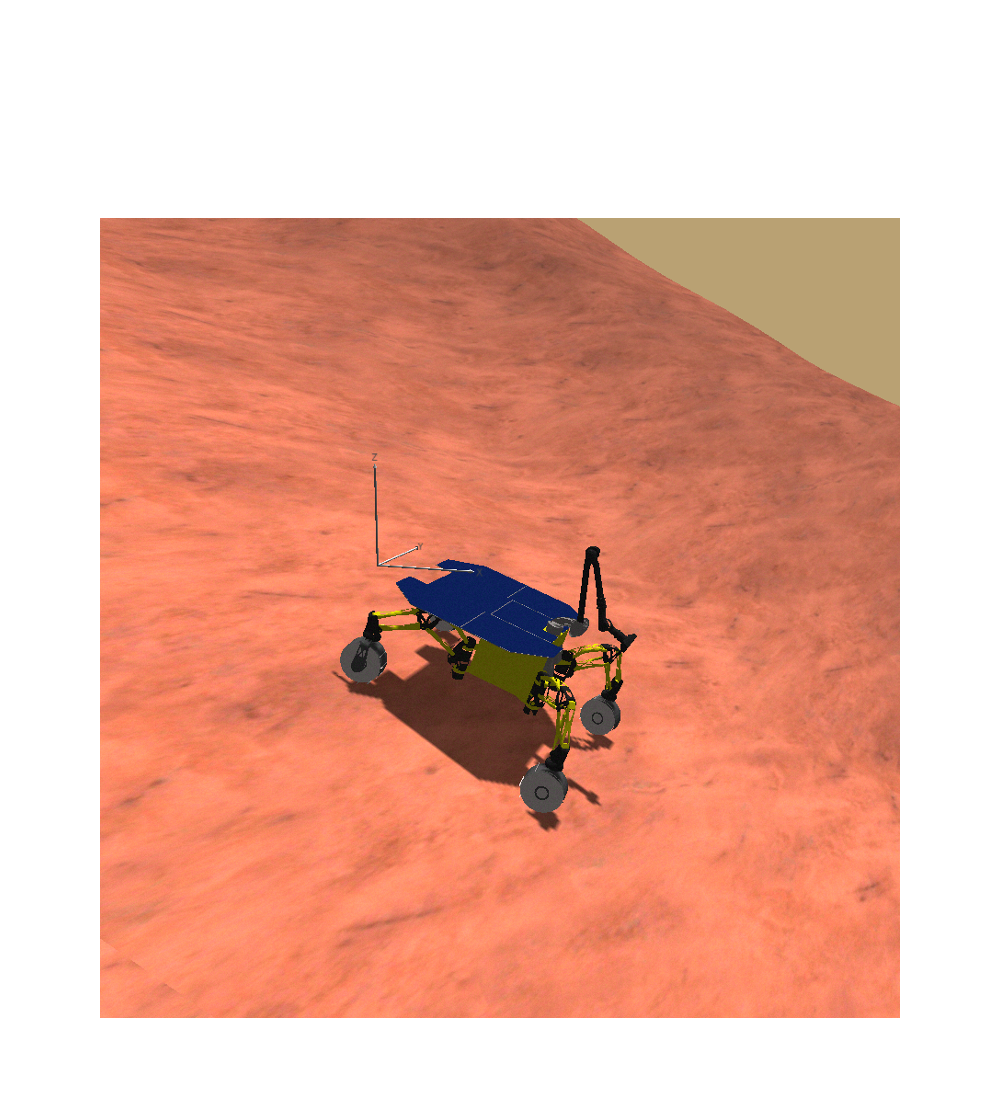
\includegraphics[height=77mm]{sections/power-system-design/simulation/images/counter-slope.png}
  		\subcaption{Simulation environment}
		\label{fig:sub:rover-slope-compensation-simulation}
    \end{subfigure}\hfill
    \begin{subfigure}[t]{\subfigureWidth}
        \centering
        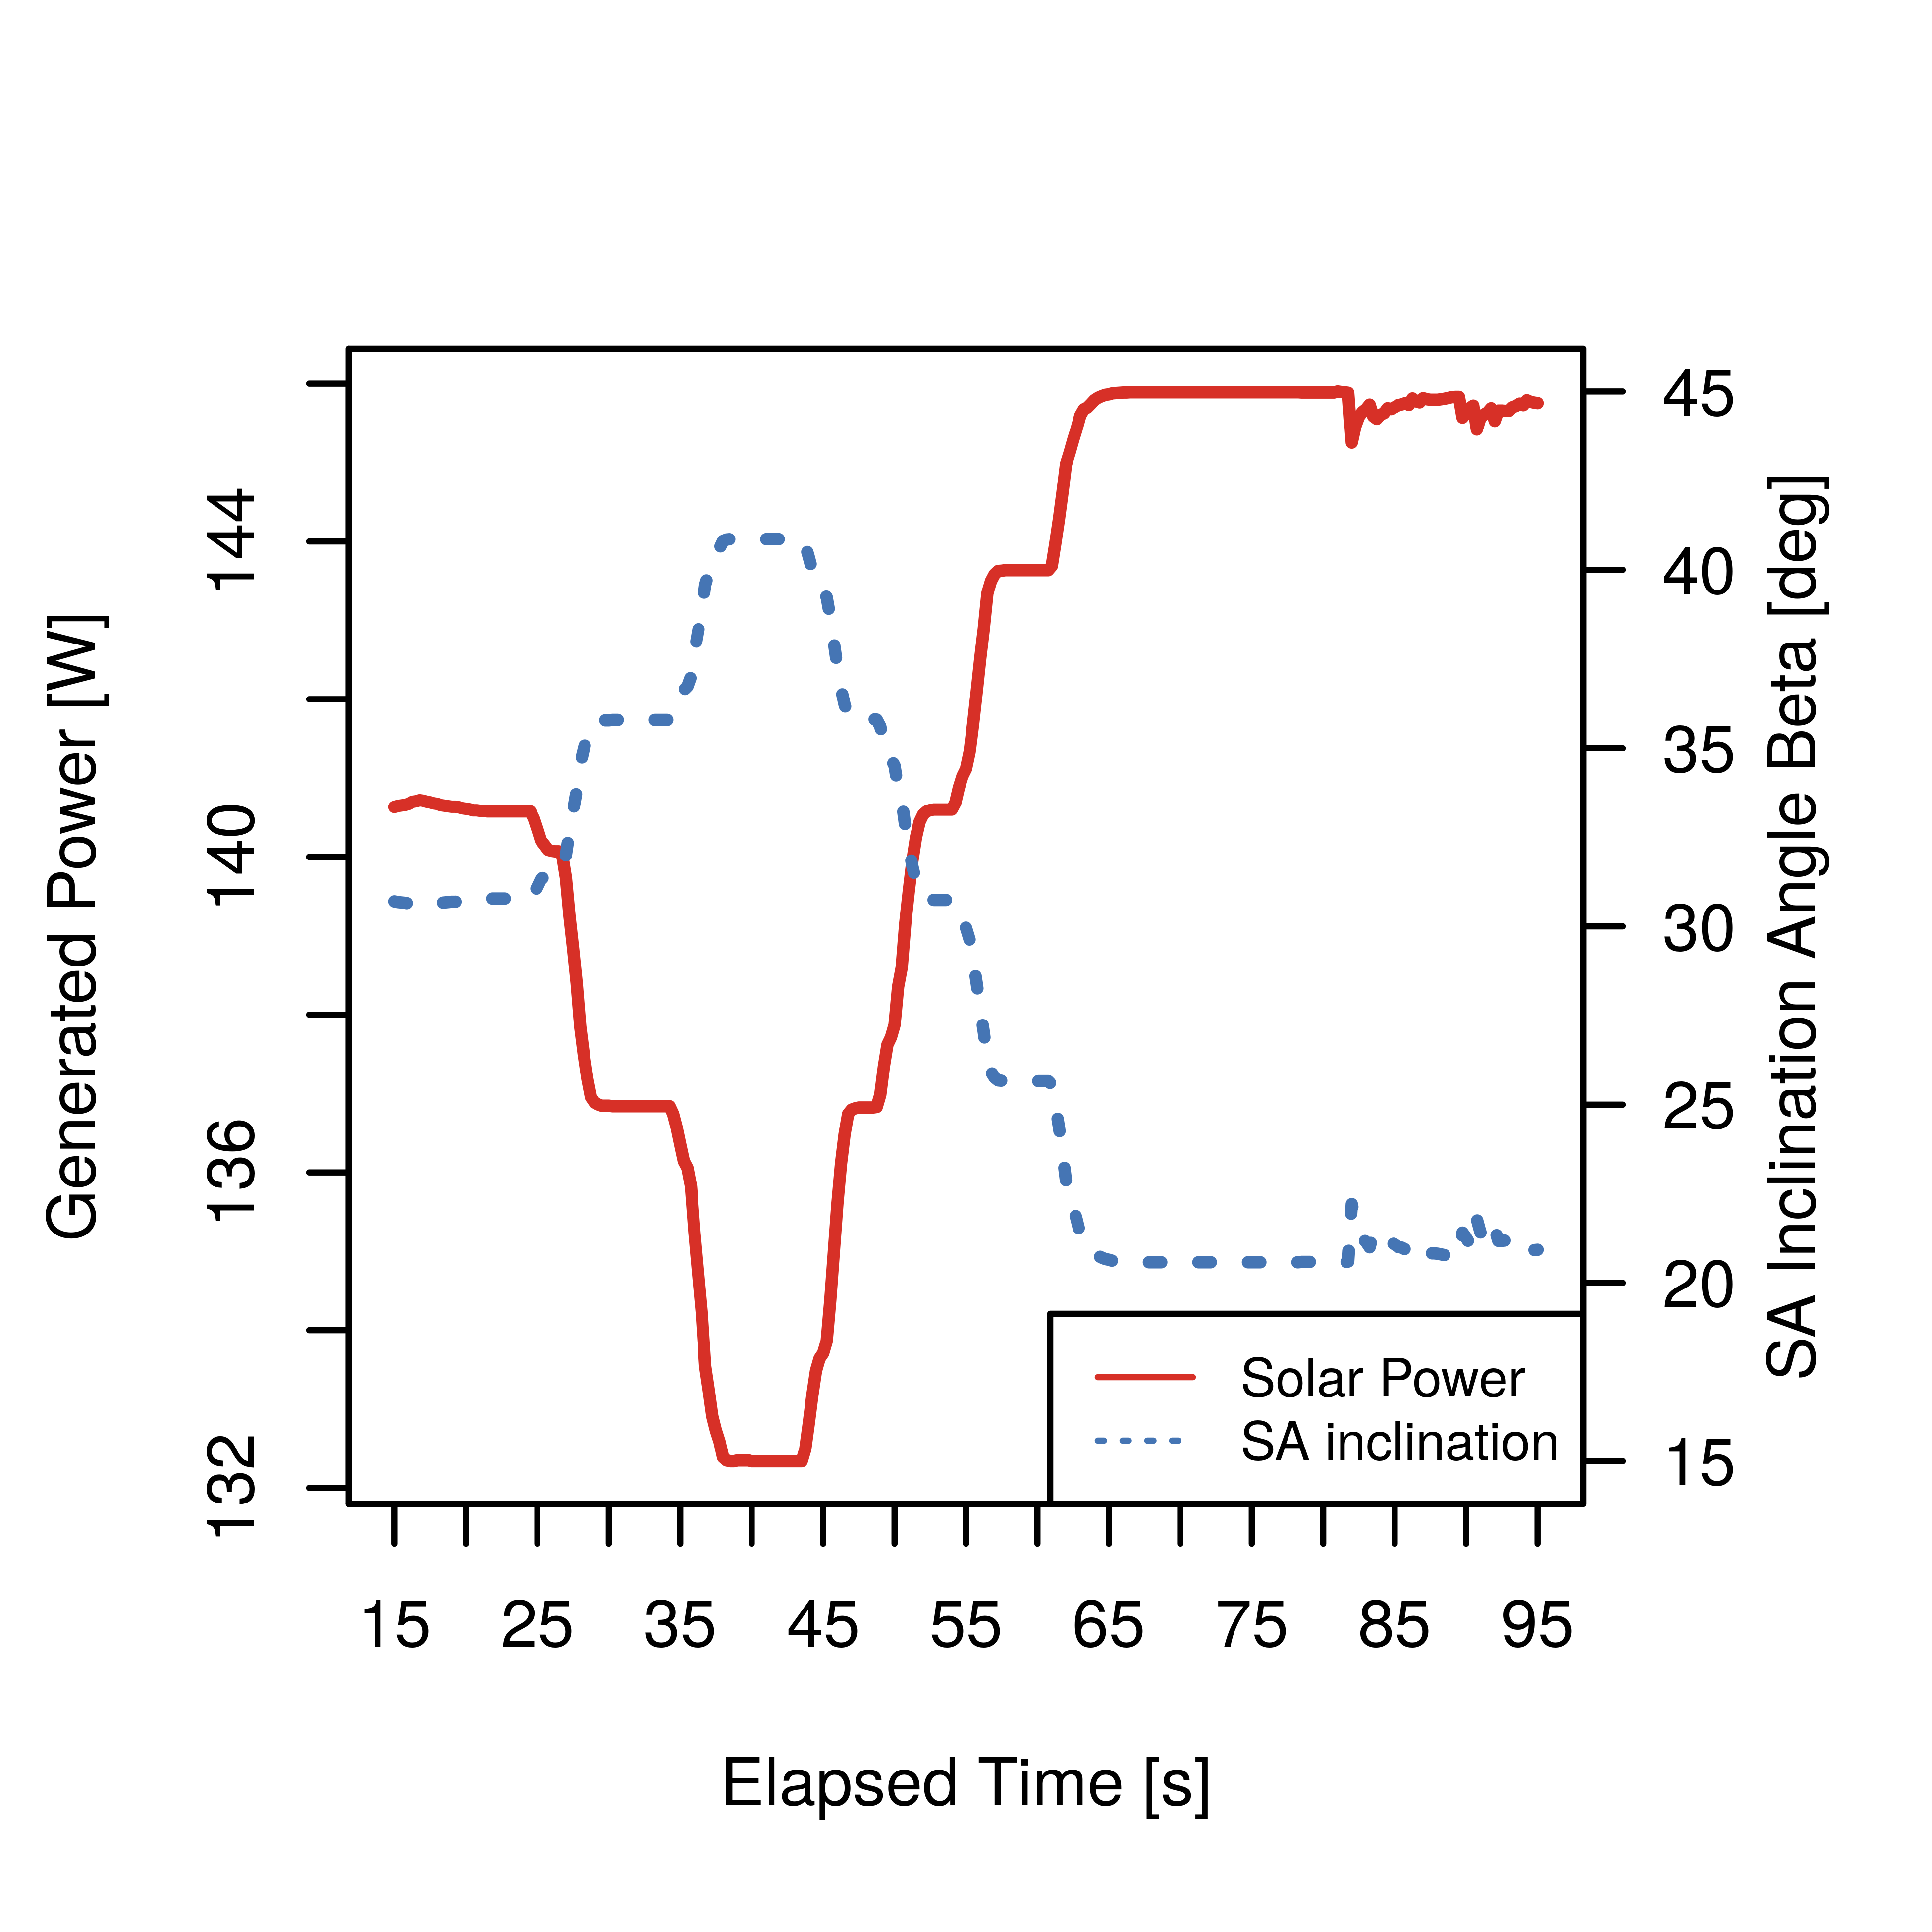
\includegraphics[height=\graphicsHeight]{sections/power-system-design/simulation/plots/slope-compensation.png}
  		\subcaption{Measurements}
		\label{fig:sub:rover-slope-compensation-power-profile}
	\end{subfigure}\\[0.8ex]
    \caption[Simulation of solar power generation on an inclined slope]
            {Simulation of solar power generation on an inclined slope at Ismenius Cavus during solar noon.}
    \label{fig:rover-slope-compensation}
\vspace{-2ex}
\end{figure}

\clearpage

\refFig{fig:sub:rover-slope-compensation-power-profile} shows solar power outputs for different body-pitch configuration while the rover is on a \SI{30}{\degree} slope. The initial state of the \ac{SA} $\beta$ inclination angle is equal to that of the slope angle. Two seperate \SI{5}{\degree} forward pitch increments are executed at \SI{25}{\second} and \SI{35}{\second} which worsen solar power output by changing \ac{SA} $\beta$ inclination angle from ~\SI{30}{\degree} to ~\SI{40}{\degree}. Following that, four separate \SI{5}{\degree} backward pitch decrements are executed from \SI{45}{\second} to \SI{65}{\second}, progressively improving power generation as $\beta$ is changed from ~\SI{40}{\degree} to ~\SI{20}{\degree}. As a final task, the rover is commanded to drive forward at \SI{80}{\second} and it encounters uneven terrain which introduces minor fluctuations to the solar power output.
